\section{Mechanics of Selective SSMs}
\label{sec:mechanics}

%

\begin{proof}[Proof of \cref{thm:gating}]
Consider a selective SSM (\cref{alg:s6}) with
$N=1, \A=-1, \B=1, s_\dt=\mathsf{Linear}(x), \tau_\dt=\mathsf{softplus}$.
The corresponding continuous-time SSM \eqref{eq:ssm} is
\begin{align*}%
  h(t) = -h(t) + x(t)
\end{align*}
which is also called a \emph{leaky integrator}.

The discretization step size is
\begin{align*}%
  \dt_t &= \tau_\dt(\mathsf{Parameter} + s_\dt(x_t)) \\
      &= \mathsf{softplus}(\mathsf{Parameter} + \mathsf{Linear}(x_t)) \\
      &= \mathsf{softplus}(\mathsf{Linear}(x_t))
\end{align*}
where we observe that the parameter can be viewed as a learnable bias and folded into the linear projection.

Now applying the zero-order hold (ZOH) discretization formulas:
\begin{align*}%
  \dA_t &= \exp(\dt \A) = \frac{1}{1 + \exp(\mathsf{Linear}(x_t))} = \sigma(-\mathsf{Linear}(x_t))
    \\&= 1 - \sigma(\mathsf{Linear}(x_t))
    \\
  \dB_t &= (\dt \bm{A})^{-1} (\exp(\dt \bm{A}) - \bm{I}) \cdot \dt \bm{B} = -(\exp(\dt \bm{A}) - \bm{I}) = 1 - \dA
    \\&= \sigma(\mathsf{Linear}(x_t))
    .
\end{align*}

Thus the final discrete recurrence \eqref{eq:ssm:recurrence:1} is
\begin{align*}%
  g_t &= \sigma(\mathsf{Linear}(x_t)) \\
  h_{t} &= (1-g_t) h_{t-1} + g_t x_t
\end{align*}
as desired.
\end{proof}

%

\section{Hardware-aware Algorithm For Selective SSMs}
\label{sec:hardware_aware_algo}

Without input-dependent selectivity, SSMs can be efficiently implemented as a
convolution~\citep{gu2022efficiently,dao2023hungry}, which leverages the fast
Fourier transform (FFT) as primitive.
With selectivity, SSMs are no-longer equivalent to convolution, but we leverage
the parallel associative scan.
While SSM scans are theoretically efficient ($O(B L D N)$ FLOPs, scaling linear
in $L$), training foundation models with selective SSMs requires them to be efficient on
modern hardware (GPUs) as well.
We describe how we use \emph{kernel fusion} and \emph{recomputation} to make SSM
scan fast and memory-efficient.
We evaluate the speed of our scan implementation compared to
convolution and attention in \cref{sec:exp:benchmark}, showing that it is up to 7$\times$
times faster than attention at sequence length 32K, and is as memory-efficient
as the best attention implementation (FlashAttention).

\paragraph{Speed.}
On modern hardware accelerators (GPUs) most operations (except matrix multiply)
are bounded by
memory-bandwidth~\citep{williams2009roofline,ivanov2021data,dao2022flashattention}.
This the case with our scan operation, and we use
kernel fusion to reduce the amount of memory IOs, leading to significant speedup
compared to a standard implementation.

The standard way to implement the scan algorithm in \cref{sec:method:selective}
is to prepare the scan input $\dA, \dB$ of size $(B, L, D, N)$ in GPU HBM
(high-bandwidth memory, commonly referred to as GPU memory), call a
parallel associative scan implementation to write the scan output of size
$(B, L, D, N)$ to GPU HBM, then multiply that scan output with $\C$ to
produce an output of size $(B, L, D)$.
However, this requires the number of memory reads/writes on the order of
$O(BLDN)$.
We can instead fuse the discretization step, the scan, and the multiplication
with $\C$ into one kernel:
\begin{enumerate}
  \item We read in $O(BLD + DN)$ bytes of memory ($\dt, \A, \B, \C$) from slow
  HBM to fast SRAM.
  \item We discretize to produce $\dA, \dB$ of size $(B, L, D, N)$ in SRAM.
  \item We perform a parallel associative scan, yielding intermediate states of
  size $(B, L, D, N)$ in SRAM.
  \item We multiply and sum with $\C$, producing outputs of size $(B, L, D)$ and
  write it to HBM.
\end{enumerate}
This way, we reduce IOs by a factor of $O(N)$ (the state dimension), which in
practice speeds up the operation by 20-40 times (\cref{sec:exp:benchmark}).

For sequence length $L$ too long where we cannot fit the sequence in SRAM (which
is much smaller than HBM), we split the sequences into chunks and perform the
fused scan on each chunk. As long as we have the intermediate scan states, we
can continue the scan with the next chunk.

\paragraph{Memory.}
We describe how we use the classical technique of \emph{recomputation} to reduce
the total amount of memory required to train selective SSM layers.

From the way we fuse the forward pass, we do not save the intermediate states of
size $(B, L, D, N)$ to avoid memory blowup.
However, these intermediate states are necessary for the backward pass to
compute gradients.
We instead recompute those intermediate states in the backward pass.
Since the inputs $\dt, \A, \B, \C$ and output gradient read from HBM to SRAM are
of size $O(BLN + DN)$, and the input gradients are also of size $O(BLN + DN)$,
recomputation avoids the cost of reading $O(BLND)$ elements from HBM.
This means that recomputation of the SSM states in the backward pass speeds up
the computation compared to storing them and reading them from HBM.

Beyond optimizing for the memory requirement of just the scan operation, we also
use recomputation to optimize the memory requirement of the entire selective SSM block (input projection,
convolution, activation, scan, output projection).
In particular, we do not save intermediate activations that take a lot of memory
but are fast to recompute (e.g. output of activation function or short
convolution).
As a result, the selective SSM layer has the same memory requirement as an optimized
Transformer implementation with FlashAttention.
In particular, each attention layer (FlashAttention) stores around 12 bytes of
activations per token, an each MLP layer stores around 20 bytes of activations
per token, for a total of 32 bytes ((assuming mixed-precision training in FP16
or BF16)).
Each selective SSM stores around 16 bytes of activations per token.
Hence two layers of selective SSMs have around the same activation memory as an
attention layer and an MLP layer.


\iftoggle{arxiv}{}{
\section{Full Experiments}

\subsection{Synthetic Tasks}
\label{sec:exp-full:synthetic}
Full experiment details for these tasks including task details and training protocol are in \cref{sec:exp-details:synthetics}.

\subsubsection{Selective Copying}


The Copying task is one of the most well-studied synthetic tasks for sequence modeling,
originally designed to test the memorization abilities of recurrent models.
As discussed in \cref{sec:method:motivation}, LTI SSMs (linear recurrences and global convolutions)
can easily solve this task by only keeping track of time instead of reasoning about the data;
for example, by constructing a convolution kernel of exactly the right length (\cref{fig:copying}).
This was explicitly validated in earlier work on global convolutions~\citep{romero2021ckconv}.
The Selective Copying task prevents this shortcut by randomizing the spacing between tokens.
Note that this task has been introduced before as the Denoising task~\citep{jing2019gated}.

Note that many previous works argue that adding architecture gating (multiplicative interactions) can endow models with ``data-dependence'' and solve related tasks \citep{dao2023hungry,poli2023hyena}.
However, we find this explanation insufficient intuitively because such gating does not interact along the sequence axis, and cannot affect the spacing between tokens.
In particular architecture gating is not an instance of a selection mechanism (\cref{sec:discussion:selection}).

\cref{tab:copying} confirms that gated architectures such as H3 and Mamba only partially improve performance,
while the selection mechanism (modifying S4 to S6) easily solves this task, particularly when combined with these more powerful architectures.



\subsubsection{Induction Heads}

Induction heads~\citep{olsson2022context} is a simple task from the mechanistic interpretability lens~\citep{elhage2021mathematical} that is surprisingly predictive of the in-context learning ability of LLMs. It requires models to perform associative recall and copy: for example, if the model has seen a bigram such as ``Harry Potter'' in the sequence, then the next time ``Harry'' appears in the same sequence, the model should be able to predict ``Potter'' by copying from history.

\paragraph{Dataset.}
We train a 2-layer model on the induction heads task at sequence length $256$, with a vocab size of $16$,
which is comparable to prior work on this task \citep{dao2023hungry} but with longer sequences.
We additionally investigate generalization and extrapolation abilities by evaluating on a range of sequence lengths from $2^6 = 64$ up to $2^{20} = 1048576$ at test time.

\paragraph{Models.}
Following established work on induction heads, we use 2 layer models, which allows attention to mechanistically solve the induction heads task~\citep{olsson2022context}.
We test both multi-head attention (8 heads, with various positional encodings) and SSM variants.
We use a model dimension $D$ of $64$ for Mamba and $128$ for the other models.

\paragraph{Results.}

\cref{fig:induction} shows that
Mamba---or more precisely, its selective SSM layer---has the ability to solve the task perfectly because of its ability to selectively remember the relevant token while ignoring everything else in between.
\textbf{It generalizes perfectly to million-length sequences, or $4000\times$ longer than it saw during training},
while no other method goes beyond $2\times$.

Out of positional encoding variants for attention models, xPos (which was designed for length extrapolation) is slightly better than the others;
also note that all attention models were only tested up to sequence length $2^{14}=16384$ due to memory limitations.
Out of other SSMs, H3 and Hyena are similar, contrary to the findings in \citet{poli2023hyena}.

%






\subsection{DNA Modeling}
\label{sec:exp-full:genomics}

For pretraining, we largely follow a standard causal language modeling (next token prediction) setup for the training and model details (see also \cref{sec:exp-details:lm}).
For the dataset, we largely follow the setup of HyenaDNA~\citep{nguyen2023hyenadna}, which uses the HG38 dataset for pretraining consisting of a single human genome
with about 4.5 billion tokens (DNA base pairs) in the training split.

\subsubsection{Scaling: Model Size}


In this experiment, we investigate the scaling properties of genomics foundation models with various model backbones (\cref{fig:dna} \textit{Left}).
%


\para{Training.}
To advantage the baselines, we train on a short sequence length of $1024$; as shown in \cref{sec:exp:dna:length}, we expect results to favor Mamba even more at longer sequence lengths.
We fix a global batch size of $1024$, for a total of $2^{20} \approx 1M$ tokens per batch.
Models were trained for $10K$ gradient steps for a total of $10B$ tokens.

\para{Results.}
\cref{fig:dna} (\emph{Left}) shows that Mamba's pretraining perplexity improves smoothly with model size,
and that Mamba scales better than both HyenaDNA and Transformer++.
For example, at the largest model size of $\approx 40M$ parameters,
the curve shows that \textbf{Mamba can match the Transformer++ and HyenaDNA models with roughly $3\times$ to $4\times$ fewer parameters}.


\subsubsection{Scaling: Context Length}
\label{sec:exp:dna:length}

In the next DNA experiment, we investigate the scaling properties of models with respect to sequence length.
We only compare the HyenaDNA and Mamba models, as quadratic attention becomes prohibitively expensive at longer sequence lengths.
We pretrain models on sequence lengths $2^{10}=1024$, $2^{12}=4096$, $2^{14}=16384$, $2^{16}=65536$, $2^{18}=262144$, $2^{20}=1048576$.
We fix a model size of 6 layers by width $128$ (about 1.3M-1.4M parameters).
Models were trained for $20K$ gradient steps for a total of $\approx 330B$ tokens.
The longer sequence lengths used sequence length warmup similar to \citep{nguyen2023hyenadna}.

\para{Results.}
\cref{fig:dna} (\emph{Right}) shows that \textbf{Mamba is able to make use of longer context even up to extremely long sequences of length 1M}, and its pretraining perplexity improves as the context increases.
On the other hand, the HyenaDNA model gets worse with sequence length.
This is intuitive from the discussion in \cref{sec:method:properties} on properties of the selection mechanism.
In particular, LTI models cannot selectively ignore information;
from a convolutional perspective, a very long convolution kernel is aggregating all information across a long sequence which may be very noisy.
Note that while HyenaDNA claims to improve with longer context, their results do not control for computation time.


\subsubsection{Synthetic Species Classification}

We evaluate models on a downstream task of classifying between 5 different species by randomly sampling a contiguous segment of their DNA.
This task is adapted from HyenaDNA,
which used the species $\{ \texttt{human}, \texttt{lemur}, \texttt{mouse}, \texttt{pig}, \texttt{hippo} \}$.
We modify the task to be significantly more challenging by classifying between the five \emph{great apes} species \\ $\{ \texttt{human}, \texttt{chimpanzee}, \texttt{gorilla}, \texttt{orangutan}, \texttt{bonobo} \}$,
which are known to share 99\% of their DNA.


\begin{table}[h]
    % \captionsetup{font=small}
    \small
    \centering
    % \vspace{-1em}
    \caption{\label{table:ablations} Perplexity of SSM variants compared to
      Transformers on OpenWebText. All models have 12 layers, with size around 125M, and are trained
      with the same hyperpameters, for 50B tokens.}
    %   \vspace{1em}
    {
        \begin{tabular}{@{}|ccccc|c|@{}}
            \hline
        %   \specialrule{.15em}{.05em}{.05em}
        \hthree & \hthree Hybrid (2 Attn) & S4D & GSS & GSS Hybrid (2 Attn) & Transformer  \\ % & Training time \\
        %   \specialrule{.15em}{.05em}{.05em}
        \hline
        21.0 & \textbf{19.6} & 24.9 & 24.0 & 19.8 & 20.6 \\ \hline
        \end{tabular}
    }
    % \vspace{-1.5em}
\end{table}

\subsection{Speed and Memory Benchmarks}
\label{sec:exp:benchmark}


We benchmark the speed of the SSM scan operation (state expansion $N=16$), as well as the end-to-end
inference throughput of Mamba, in \cref{fig:scan_benchmark}.
Our efficient SSM scan is faster than the best attention implementation that we know of
(FlashAttention-2~\citep{dao2023flashattention2}) beyond sequence length 2K,
and up to 20-40$\times$ faster than a standard scan implementation in
PyTorch.
Mamba achieves 4-5$\times$ higher inference throughput than a Transformer of similar
size, since without the KV cache it can use much higher batch sizes.
For example, a Mamba-6.9B (untrained) would have higher inference throughput than a
$5\times$ smaller Transformer-1.3B.
Details in \cref{sec:exp-details:benchmark}, which additionally includes a benchmark of memory consumption.

}


\section{Experimental Details and Additional Results}
\label{sec:exp-details}


\subsection{Synthetic Tasks}
\label{sec:exp-details:synthetics}

\paragraph{Selective Copying.}

Our setting is on sequences of length 4096, with a vocab size of 16 possible tokens (including the white ``noise'' token from \cref{fig:copying}) and requiring models to memorize 16 ``data'' tokens.
We use 2 layer models with a model dimension of $D = 64$.

Models are trained for 400K steps
at a constant learning rate of $0.0001$
with a batch size of $64$.

\paragraph{Induction Heads.}

\begin{table}
  \footnotesize
  \caption{
    (\textbf{Induction heads}.)
    Models are trained on sequence length $2^8=256$, and tested on various sequence lengths of $2^6=64$ up to $2^{20}=1048576$.
    \cmark\ denotes perfect generalization accuracy, while \xmark\ denotes out of memory.
  }
  \centering
  \begin{tabular}{@{}lllllllllllllllll@{}}
    \toprule
    \sc{Model}       & \sc{Params} & \multicolumn{15}{c}{\sc{Test Accuracy (\%) at Sequence Length}} \\
    \cmidrule(lr){3-17}
                &        & $2^6$  & $2^7$  & $\bm{2^8}$ & $2^9$     & $2^{10}$ & $2^{11}$   & $2^{12}$  & $2^{13}$   & $2^{14}$ & $2^{15}$ & $2^{16}$ & $2^{17}$ & $2^{18}$ & $2^{19}$ & $2^{20}$ \\
    \midrule
    MHA-Abs     & 137K   & \cmark & 99.6   & 100.0      & 58.6      & 26.6     & 18.8       & 9.8       & 10.9       & 7.8      & \xmark   & \xmark   & \xmark   & \xmark   & \xmark   & \xmark \\
    MHA-RoPE    & 137K   & \cmark & \cmark & 100.0        & 83.6      & 31.3     & 18.4       & 8.6       & 9.0        & 5.5      & \xmark   & \xmark   & \xmark   & \xmark   & \xmark   & \xmark \\
    MHA-xPos    & 137K   & \cmark & \cmark & 100.0      & 99.6      & 67.6     & 25.4       & 7.0       & 9.0        & 7.8      & \xmark   & \xmark   & \xmark   & \xmark   & \xmark   & \xmark \\
    H3          & 153K   & \cmark & \cmark & 100.0      & 80.9      & 39.5     & 23.8       & 14.8      & 8.2        & 5.9      & 6.6      & 8.2      & 4.7      & 8.2      & 6.3      & 7.4 \\
    Hyena       & 69M$^*$    & 97.7   & \cmark & 100.0      & \cmark    & 44.1     & 12.5       & 6.6       & 5.1        & 7.0      & 5.9      & 6.6      & 6.6      & 5.9      & 6.3      & 9.8 \\
    Mamba       & 74K    & \cmark & \cmark & 100.0      & \cmark    & \cmark   & \cmark     & \cmark    & \cmark     & \cmark   & \cmark   & \cmark   & \cmark   & \cmark   & \cmark   & \cmark \\
    \bottomrule
    \multicolumn{17}{l}{\begin{tabular}{@{}l@{}}\footnotesize{$^*$ Most of the parameters are in learnable positional encodings.}\end{tabular}}
  \end{tabular}
  \label{tab:induction}
\end{table}


Training consists of randomly generating data every step, with a batch size of $8$.
We choose an ``epoch'' size of 8192 steps, and track the accuracy on fixed validation sets (also randomly generated) of each target sequence length. %
For the MHA-Abs and Mamba models, results are reported after the 25th epoch ($8192 \times 25 = 204800$ steps).
For the MHA-RoPE and MHA-xPos models, results are reported after the 50th epoch ($8192 \times 50 = 409600$ steps).
For the LTI H3 and Hyena models, results are reported after the 10th epoch ($81920$ steps) because they had converged by then and failed to improve further.

We use the Adam optimizer with no weight decay.
All models are trained at constant learning rates $2e-4$ and $1e-3$,
and the better results are reported for each model ($2e-4$ for all models except Mamba).
The attention and Hyena models did not learn at LR $1e-3$.
H3 learned at both LRs, but interestingly generalized better to shorter sequences at the smaller LR of $2e-4$.
Mamba learned at both LRs, but extrapolated better at the larger LR of $1e-3$.


\subsection{Language Modeling}
\label{sec:exp-details:lm}


\subsubsection{Scaling Law Details}
\label{sec:exp-details:lm:scaling}

Scaling law experiments generally followed the GPT3 recipe.
All models were trained on the Pile with the GPT2 tokenizer.

\paragraph{Model Sizes.}

\cref{tab:gpt3} specifies the model sizes we use for scaling laws.
This is taken directly from the GPT3 specifications~\citep{brown2020language},
with very minor modifications.
First, we changed the batch size of the 1.3B model from 1M tokens to 0.5M tokens, since we did not use enough parallelization to require the larger batch size.
Second, we changed the number of training steps and total tokens to roughly match Chinchilla scaling laws~\citep{hoffmann2022empirical}, which specify that training tokens should increase proportionally to model size.

\begin{table}
  \caption{
    (\textbf{Scaling Law Model Sizes}.)
    Our model sizes and hyperparameters for scaling experiments.
    (Model dimension and number of heads applies only to Transformer models.)
  }
  \centering
  \small
  \begin{tabular}{@{}llllllll@{}}
    \toprule
    \sc{Params} & $\mathtt{n\_layers}$ & $\mathtt{d\_model}$ & $\mathtt{n\_heads}$ / $\mathtt{d\_head}$ & \sc{Training steps}  & \sc{Learning Rate}  & \sc{Batch Size} & \sc{Tokens} \\
    \midrule
    125M   & 12                   & 768                 & 12 / 64                                  & 4800            & 6e-4           & 0.5M tokens & 2.5B       \\
    350M   & 24                   & 1024                & 16 / 64                                  & 13500           & 3e-4           & 0.5M tokens & 7B         \\
    760M   & 24                   & 1536                & 16 / 96                                  & 29000           & 2.5e-4         & 0.5M tokens & 15B       \\
    1.3B   & 24                   & 2048                & 32 / 64                                  & 50000           & 2e-4           & 0.5M tokens & 26B       \\
    \bottomrule
  \end{tabular}
  \label{tab:gpt3}
\end{table}

\paragraph{Training Recipes.}

All models used the AdamW optimizer with
\begin{itemize}
  \item gradient clip value $1.0$
  \item weight decay $0.1$
  \item no dropout
  \item linear learning rate warmup with cosine decay
\end{itemize}
By default, the peak learning rate is the GPT3 specification.

We give several models an ``improved recipe'', inspired by changes adopted by popular large language models such as PaLM~\citep{chowdhery2022palm} and LLaMa~\citep{touvron2023llama}.
These include:
\begin{itemize}
  \item linear learning rate warmup with cosine decay to $1e-5$, with a peak value of $5\times$ the GPT3 value
  \item no linear bias terms
  \item RMSNorm instead of LayerNorm
  \item AdamW hyperparameter $\beta=(.9, .95)$ (the GPT3 value) instead of the PyTorch default of $\beta=(.9, .999)$
\end{itemize}

\paragraph{Architecture and Training Details.}

Our models are:
\begin{itemize}[leftmargin=*,itemsep=0pt]
  \item \textbf{Transformer}: The standard Transformer based on GPT3 (\cref{tab:gpt3}).
  \item \textbf{Transformer++}: A Transformer with an improved architecture, namely rotary positional encodings \citep{su2021roformer} and SwiGLU MLP~\citep{shazeer2020glu}, and the improved training recipe above.
  \item \textbf{Hyena}: Interleaving a Hyena block (the H3 block with S4 replaced by a global convolution parameterized by an MLP) with standard MLP blocks.
    The MLP blocks have expansion factor $2$ instead of $4$ and the number of layers is correspondingly increased by $1.5\times$ to preserve parameter count.
  \item \textbf{H3++}: The H3 architecture with a few modifications, including (i) using the same ``thin'' Hyena dimensions above (ii) the improved training recipe above (iii) a linear attention \emph{head dimension} of 8.
  \item \textbf{RWKV}: The default RWKV model from \citet{peng2023rwkv}, including its modified MLP block. We also used as much of its specified training recipe as possible, such as increasing the learning rates by $2\times$ or $3\times$ on certain parameters.
  \item \textbf{RetNet}: The default RetNet model from~\citet{sun2023retentive}. We also gave it the improved training recipe above.
  \item \textbf{Mamba}: The standard Mamba architecture, with the improved training recipe.
\end{itemize}

\subsubsection{Additional Scaling Law Ablations}
\label{sec:exp-details:lm:scaling-ablations}

We perform additional ablations on the architecture using the same protocol as the 2k context length scaling laws in \cref{fig:lm-scaling} (\emph{Left}).

\paragraph{Mamba Architecture: Interleaving Blocks.}

We test the effect of different architectural blocks combined with the Mamba block.
We focus on the viewpoint that the Mamba block is simply the standard SwiGLU block with an extra $\mathsf{conv} \to \mathsf{SSM}$ path added.
This leads to two natural ablations:
\begin{itemize}[leftmargin=*,itemsep=0pt]
  \item What if the Mamba block is interleaved with a standard MLP block, instead of stacked homogenously? This can also be interpreted as taking Mamba and removing half of the SSMs.
  \item What if the Mamba block is interleaved with MHA (multi-head attention) blocks? This can also be interpreted as taking a Transformer with SwiGLU MLPs (i.e.\ what we call Transformer++) and simply adding SSMs to the MLP blocks.
\end{itemize}

\cref{fig:lm-scaling-ablations} (\emph{Right}) shows these variants compared to the original (homogenous) Mamba architecture.
Interestingly, neither change matters too much.
The Mamba-MLP architecture is only slightly worse, and still better than all models except Transformer++.
The Mamba-MHA architecture is only slightly better, which is somewhat surprising in light of the fact that many recent works
have found that combining (LTI) SSMs with Attention can lead to substantial improvements~\citep{dao2023hungry,fathullah2023multi,saon2023diagonal,zuo2022efficient,fathi2023block}.


\paragraph{H3 Architecture: Training Recipes.}

Next we ablate differences between the Hyena and H3++ models, our weakest and strongest models outside of Transformer++ and Mamba,
particularly to isolate the effect of training recipes.

\begin{itemize}[leftmargin=*,itemsep=0pt]
  \item \textbf{Hyena}: The Hyena block with its original architecture and GPT3 training recipe (same as \cref{fig:lm-scaling}).
  \item \textbf{Hyena+}: The same architecture but with the improved training recipe described above.
  \item \textbf{H3+}: The same architecture as Hyena+ but with the Hyena convolution kernel swapped out for S4D convolution kernel.
  \item \textbf{H3++}: The same as H3+, but with a linear attention \emph{head dimension} of 8. This increases computation inside the SSM recurrence but does not increase parameters.
\end{itemize}

Our general convention is that ``Model+'' represents the base model with the improved training recipe,
and ``Model++'' also allows for architectural changes.

\cref{fig:lm-scaling-ablations} (\emph{Right}) shows that
\begin{itemize}[leftmargin=*,itemsep=0pt]
  \item A large improvement is achieved by the improved training recipe, which was used for many of the models in the main \cref{fig:lm-scaling} (RetNet, H3++, Transformer++, Mamba).
  \item The choice of the inner LTI SSM does not matter (e.g.\ Hyena vs.\ S4), consistent with findings throughout this paper.
  \item The head dimension expansion improves performance, consistent with one of our main themes that expanded state dimension improves performance for SSMs (\cref{sec:method}).
\end{itemize}


\begin{figure}[!t]
  \centering
  \begin{subfigure}[t]{0.49\linewidth}
    \centering
    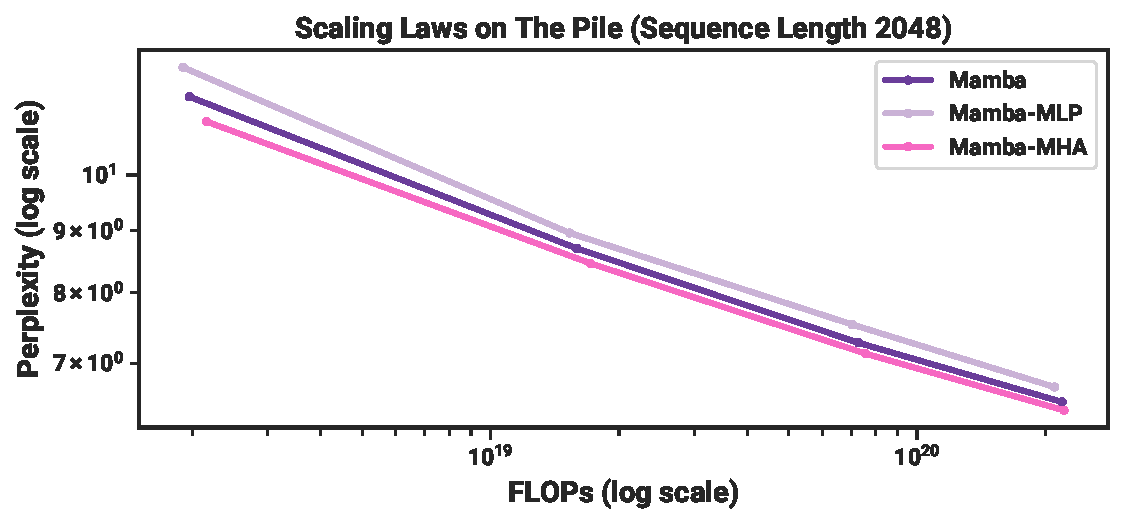
\includegraphics[width=\textwidth]{fig/pile_2k_ablations_mamba.pdf}
  \end{subfigure}
  \begin{subfigure}[t]{0.49\linewidth}
    \centering
    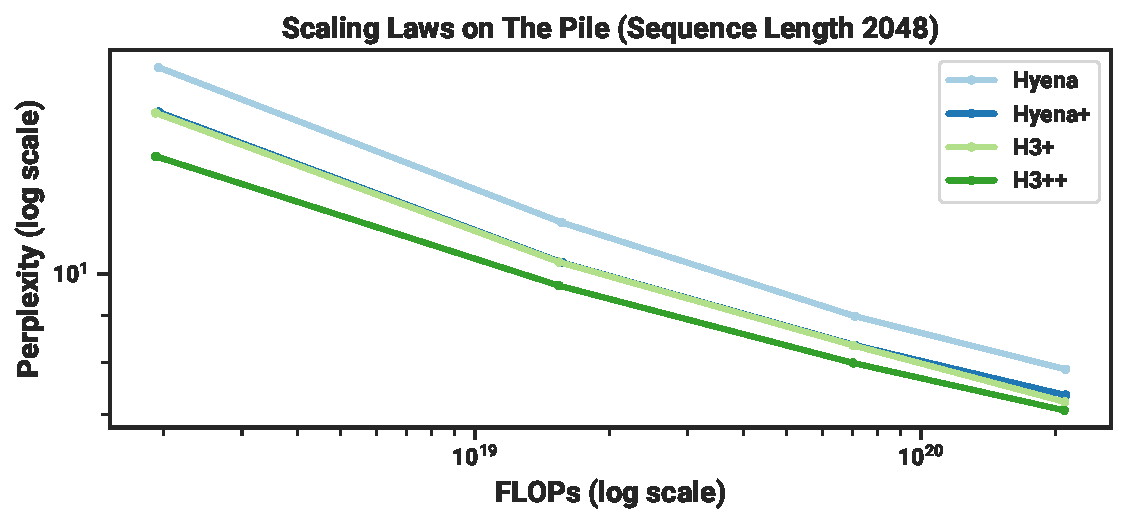
\includegraphics[width=\textwidth]{fig/pile_2k_ablations_h3.pdf}
  \end{subfigure}
  \caption{
    (\textbf{Scaling laws: extra ablations}.) %
    (\emph{Left}) Instead of 
    (\emph{Right}) Instead of 
  }
  \label{fig:lm-scaling-ablations}
\end{figure}

%

%

\subsubsection{Downstream Evaluation Details}

This pretraining procedure is the same as the scaling law protocol, but extended to 300B tokens and with the GPT-NeoX tokenizer~\citep{black2022gpt} instead of GPT2 tokenizer.
For the 1.3B model, we use a batch size of 1M tokens to be consistent with the GPT3 specifications.
We report the perplexity on the Pile validation set, and for this metric only compare to models trained on the same dataset and with the same tokenizer, in particular Pythia and RWKV.

For downstream evaluation, we use the LM evaluation harness from EleutherAI~\citep{eval-harness}, as done by most work in this area.
We evaluate on the following tasks/datasets that measure common sense reasoning:
\begin{itemize}
  \item LAMBADA~\citep{paperno2016lambada}
  \item HellaSwag~\citep{zellers2019hellaswag}
  \item PIQA~\citep{bisk2020piqa}
  \item ARC-challenge~\citep{clark2018think}
  \item ARC-easy: an easy subset of ARC-challenge
  \item WinoGrande~\citep{sakaguchi2021winogrande}
\end{itemize}

We report accuracy for LAMBADA, WinoGrande, PIQA, and ARC-easy, and accuracy normalized by sequence length for HellaSwag and ARC-challenge (since normalized accuracy is higher for almost all models for these task).

\subsection{DNA Modeling}

\subsubsection{Pretraining Details}

We describe the dataset and training procedure of the HG38 pretraining task in more detail.

The dataset follows the splits from the prior Enformer work on genomics~\citep{avsec2021effective}; the training split contains a total of $S=34021$ segments of length $2^{17}=131072$ that cover the genome,
for a total of approximately 4.5 billion tokens (DNA base pairs).
These segments are pairs of (chromosome number, starting index, ending index), and can be extended if necessary (e.g.\ to get longer segments).

We deviate from HyenaDNA when the training sequence length is not $2^{17}$.
HyenaDNA always takes a fixed sub-segment (e.g. the beginning or middle of the prescribed segment), and thus for any training sequence length each epoch is fixed to $34021$ samples and doesn't necessarily go through the whole genome.
On the other hand, we use the entire training data:
\begin{itemize}[leftmargin=*,topsep=0pt]
  \item When the context length $L$ is less than (or equal to) $2^{17}$, we divide up each segment into non-overlapping sub-segments of length $L$, so that there are $S \times \frac{2^{17}}{L}$ total samples and $S \times 2^{17} \approx 4.5B$ tokens per epoch.
  \item When the context length $L$ is greater than $2^{17}$, we turn each segment into two samples, one that begins with the prescribed segment and one that ends with the prescribed segment. Thus each epoch has $2S$ items and $2SL$ tokens per epoch. For example, at sequence length $2^{18}=262144$ there are $4\times$ as many tokens as the default, and at sequence length $2^{20}$ there are $16\times$ as many tokens.
\end{itemize}


Other training details generally follow the same protocol as our language modeling experiments (\cref{sec:exp-details:lm}).
For example, we use the AdamW with $(\beta_1, \beta_2) = (0.9, 0.95)$, no dropout, weight decay $0.1$.
We use a cosine learning rate scheduler with linear warmup for 10\% of total steps.

\subsubsection{Scaling: Model Size Details}

\paragraph{Models.}
The models we consider are:
\begin{itemize}[leftmargin=*,itemsep=0pt]
  \item Transformer++: a Transformer with improved architecture, notably the usage of RoPE positional encodings~\citep{su2021roformer}. Informally, we found these to be noticeably better than vanilla positional encodings from~\citep{vaswani2017attention}.
  \item HyenaDNA: the Hyena model from \citet{poli2023hyena,nguyen2023hyenadna}, which is roughly a Transformer with the MHA block replaced by an H3 block using a global convolution parameterized by an MLP.
  \item Mamba: the standard Mamba architecture.
\end{itemize}

\paragraph{Model Sizes.}
We use the following model sizes.
\begin{center}
  \begin{tabular}{@{}llllllll@{}}
    \toprule
    \sc{Blocks} & 4 & 5 & 6 & 7 & 8 & 10 & 12 \\
    \sc{Model Dimension} & 64 & 96 & 128 & 192 & 256 & 384 & 512 \\
    \sc{Params (Approx.)} & 250K & 700K & 1.4M & 3.5M & 7.0M & 19.3M & 40.7M \\
    \bottomrule
  \end{tabular}
\end{center}
Note that the number of blocks for Mamba is doubled, because one Transformer ``layer'' includes both the MHA and MLP blocks (and similarly for Hyena),
which requires two Mamba blocks to match parameters (\cref{sec:method:architecture}).

\paragraph{Training.}
For each model (Transformer++, HyenaDNA, Mamba), we swept the learning rate across $\{1e-3, 2e-3, 4e-3, 8e-3\}$.
The optimal Transformer and HyenaDNA learning rates were 2e-3 across all sizes.
The optimal Mamba learning rate was 8e-3; note that Mamba performed better than baselines with matched learning rates (2e-3),
but was more stable and improved even more at higher learning rates.
(Furthermore, as this LR is on the upper range of the sweep, it is possible that our results are still suboptimal.)

Note that, in contrast to standard LM scaling laws (\cref{tab:gpt3}), our LR held constant across model sizes for simplicity.
The optimal LR should go down for larger models, but we didn't find a noticeable effect at the small model sizes (at most a few million parameters) we considered.

\subsubsection{Scaling: Context Length Details}

We use a total batch size of $2^{24}\approx 16M$ tokens per training step, for every sequence length (e.g.\ at length $2^{20}$ there are $16$ segments per batch and at length $2^{10}$ there are $16384$ segments per batch).
This is a large batch size relative to the model size by usual LM standards, but
note that a batch size of $2^{23}$ is the minimum possible on a machine with 8 GPUs and sequence length of $2^20$,
and that HyenaDNA used much larger batches of $2^{28}$.

The learning rate used was $0.008$ for Mamba and 0.001 for HyenaDNA;
we initially attempted to use the same learning rate of $0.002$ from the previous section for HyenaDNA, but found that it was unstable at the longest context length.

\paragraph{Sequence Length Warmup.}
Following~\citep{nguyen2023hyenadna}, we use sequence length warmup (SLW) during pretraining.
We choose a simple schedule of 2 epochs at each power-of-two sequence length starting from $2^{10}=1024$.
(Note that because of how data is curated, at the longest sequence lengths more steps and tokens are spent proportionally.
In particular, each stage up to length $2^{17}$ processes the same number of tokens,
but $4\times$ as many tokens are processed at length $2^{18}$, $8\times$ as many at length $2^{19}$, and $16\times$ as many at length $2^{20}$.)

Unlike HyenaDNA, we always control for the number of tokens per gradient update,
so the batch size is successively halved as the sequence lengths are doubled in each stage.

\begin{remark}
  We also note that the schedule was not tuned, and we never experimented with turning off sequence length warmup for these pretraining experiments.
  We later found that SLW did not help noticeably for audio pretraining at similar lengths (\cref{sec:exp:audio}), and it is possible that it is not necessary for DNA pretraining either.
\end{remark}

\subsubsection{Species (Great Apes) Classification}

Models are causal and therefore only the last element (across the sequence length) of the model's output is used for the classification head.
Note that we control for the total number of elements in the loss function per gradient step.
The pretraining objective includes all positions across the sequence length,
so that $\mathtt{batch\_size} \times \mathtt{sequence\_length}$ is held constant; in other words, the batch size decreases as the sequence length increases.
However, for a classification task, since only the last position enters the loss,
the batch size itself is held constant.
Note that this also means that fine-tuning models with longer sequence lengths is more computationally expensive.

Training consists of 10 epochs, each of which has 1024 gradient steps.
Each gradient step uses batch size 64, which are all independently randomly drawn by uniformly picking a species, uniformly picking a chromosome, and then uniformly picking a contiguous segment of DNA.

Following~\citep{nguyen2023hyenadna}, models with a maximum context length greater than $2^{14} = 16384$ use sequence length warmup with 1 epoch at length $2^{14}=16384$, 1 epoch at length $2^{15}=32768$, 1 epoch at length $2^{16}=65536$, and so on up to the maximum sequence length.
For example, the model with $2^{20}=1048576$ context undergoes $6$ epochs of sequence length warmup before $4$ more epochs at its maximum sequence length.

The learning rate for all Hyena models is $\mathtt{4e-5}$,
while the learning rate for all Mamba models is $\mathtt{1e-4}$.
These were found by performing learning rate sweeps for each model among $\{1e-5, 2e-5, 4e-5, 1e-4, 2e-4\}$ for the smaller sequence lengths $(2^{10}, 2^{12}, 2^{14}, 2^{16})$,
and these values were consistently found to be the best for each model.
An abridged learning rate sweep was done at length $2^{18}$, which agreed with these values,
and a single run at length $2^{20}$ was performed (as described above, the computational cost of these experiments is proportional to the sequence length).
The learning rate followed a cosine decay schedule with warmup with 5 epochs of linear warmup to the maximum learning rate, and 5 epochs of cosine decay down to $1e-6$.
The unusually long learning rate warmup schedule was chosen because the sequence length warmup was also long (e.g.\ comprising 6 out of 10 epochs for the model with context length $2^{20}$); we did not experiment with this choice.

Results for the Species classification task are in \cref{tab:species}.

\begin{table}[!t]
  \caption{
    (\textbf{Great Apes DNA Classification}.)
    Accuracy after fine-tuning on sequences of length $2^{10}=1024$ up to $2^{20}=1048576$ using pretrained models of the same context length.
    Random guessing is 20\%.
  }
  \centering
  \begin{tabular}{@{}llllllll@{}}
    \toprule
    \sc{Model}         & \sc{Params}    & \multicolumn{6}{c}{\sc{Accuracy (\%) at Sequence Length}} \\
    \cmidrule(lr){3-8}
                       &                & $2^{10}$ & $2^{12}$ & $2^{14}$ & $2^{16}$ & $2^{18}$ & $2^{20}$ \\
    \midrule
    HyenaDNA           & 1.4M           & 28.04    & 28.43    & 41.17    & 42.22    & 31.10    & 54.87 \\
    Mamba              & 1.4M           & 31.47    & 27.50    & 27.66    & 40.72    & 42.41    & \textbf{71.67} \\
    \midrule
    Mamba              &  7M            & 30.00    & 29.01    & 31.48    & 43.73    & 56.60    & \textbf{81.31} \\
    \bottomrule
  \end{tabular}
  \label{tab:species}
\end{table}


\subsection{Audio Details}
\label{sec:exp-details:audio}

%

\subsubsection{YouTubeMix Audio Pretraining}

%

%

%


\paragraph{Model.}
We use a model with 3 blocks per stage ($3\times5=15$ total Mamba blocks), pooling factor $p=16$, and outer dimension $D=64$, for about 3.5M parameters.

\paragraph{Dataset.}
The data is mu-law encoded at 8 bits, so the model is modeling discrete tokens with a vocab size of $256$.

%
The dataset consists of clips of up to 1 minute long, or length $960000$,
which is subsampled and divided into segments of any desired sequence length.
Since the architecture involves two stages of pooling by a factor of $16$,
and we want the resulting sequence length to be a a multiple of $8$ for hardware efficiency,
the longest possible sequence is $468 \times 2048 = 958464$.
The rest of our sequence lengths are defined by successively halving this and rounding up to the nearest multiple of $2048$.

\cref{tab:youtubemix-lengths} lists the specifications used in \cref{fig:youtubemix}.
Beyond the varying batch sizes, the number of valid segments in the training set varied
between different sequence lengths (e.g.\ the number of training steps per epoch was not constant for different points in the graph), which may have contributed to kinks in the scaling curves.

\begin{table}[!t]
  \caption{YouTubeMix length scaling sequence lengths and batch sizes.}
  \centering
  \begin{tabular}{@{}rll@{}}
    \toprule
    \sc{Sequence length} & \sc{Batch size} & \sc{Tokens / batch} \\
    \midrule
    $468 \times 2048 = 958464$ & $1$ & $958464$ \\
    $234 \times 2048 = 479232$ & $2$ & $958464$ \\
    $117 \times 2048 = 239616$ & $4$ & $958464$ \\
    $59 \times 2048 = 120832$ & $8$ & $966656$ \\
    $30 \times 2048 = 61440$ & $16$ & $983040$ \\
    $15 \times 2048 = 30720$ & $32$ & $983040$ \\
    $8 \times 2048 = 16384$ & $64$ & $1048576$ \\
    $4 \times 2048 = 8192$ & $128$ & $1048576$ \\
    \bottomrule
  \end{tabular}
  \label{tab:youtubemix-lengths}
\end{table}

\paragraph{Training.}
Models were trained for $200K$ training steps with a maximum learning rate of $0.002$,
$20K$ (10\%) warmup steps, and weight decay $0.1$ (similar to our general pretraining recipe across domains).

\paragraph{Additional Ablations: SSM Parameterizations.}

We investigate SSM parameterizations on long-form audio waveform pretraining in the setting of \cref{fig:youtubemix}.
The setting is modified slightly to use larger models ($8$ layers and $D=64$ for 6M params, the SaShiMi default),
shorter sequences ($2^{11}=2048$ to $2^{18}=262144$ instead of $2^{13}$ to $2^{20}$), lower LR ($0.001$ from $0.002$),
and shorter training cycles (100K instead of 200K steps).

\cref{fig:youtubemix-ablations} shows that the change from S4 $\to$ S6 (i.e.\ the selection mechanism) is not always beneficial.
On long-form audio waveforms, it in fact significantly hampers performance, which may be intuitive from the point of view that audio is uniformly sampled and very smooth,
and therefore benefits from continuous linear time-invariant (LTI) methods.
After ablating away the selection mechanism, note that the resulting model is the S4 layer inside the Mamba block.
To disambiguate, we call this Mamba-S4 as opposed the default Mamba architecture Mamba-S6.

However, on the right side, we keep the outer layers of the U-Net Mamba-S4 and ablate only the inner layers.
The performance differences shrink dramatically; this reinforces the hypothesis that layers closer to the \emph{raw} audio signal should be LTI,
but once they are ``tokenized'' and compressed by the outer layers, the inner layers no longer need to be LTI.
In this setting however, the real-valued SSM still underperforms the complex-valued one.

\begin{figure}
  \begin{minipage}[t]{.49\linewidth}
    \centering
    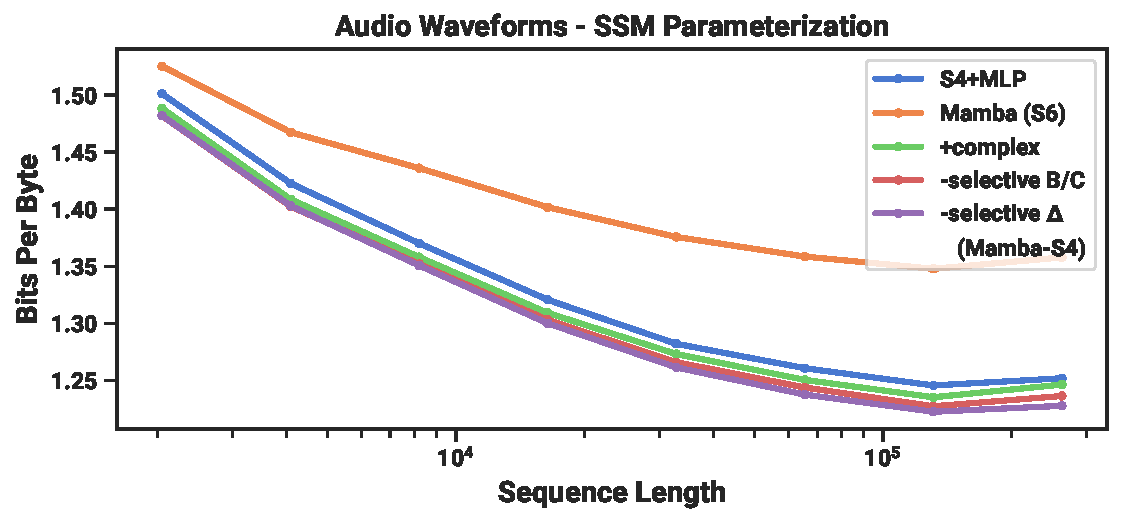
\includegraphics[width=\linewidth]{fig/youtubemix_ablations.pdf}
  \end{minipage}
  \hfill
  \begin{minipage}[t]{.49\linewidth}
    \centering
    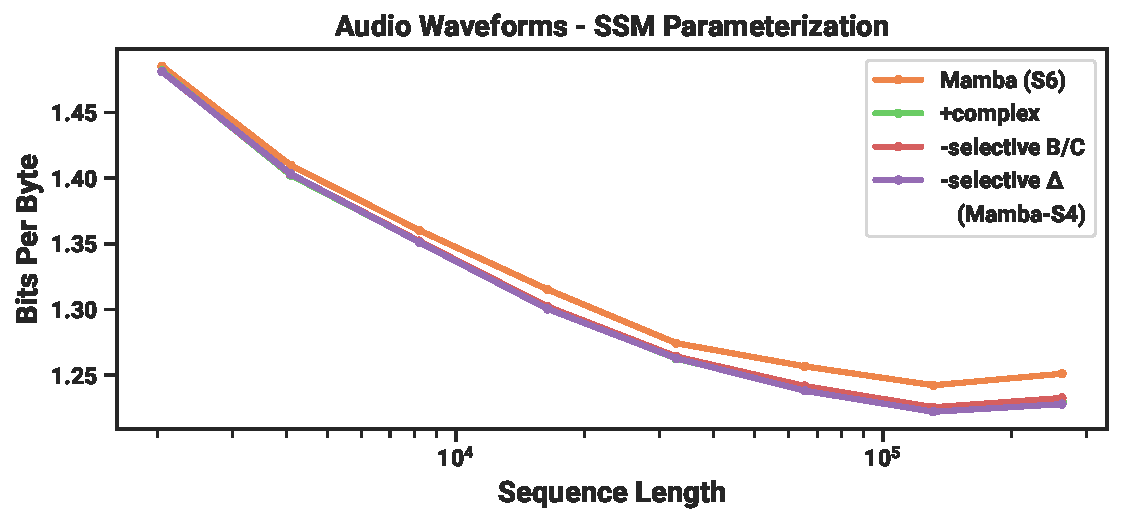
\includegraphics[width=\linewidth]{fig/youtubemix_ablations_center.pdf}
  \end{minipage}
  \captionsetup{type=figure}
  \caption{
    (\textbf{Audio Pretraining (YouTubeMix) Ablations}.)
    As a uniformly-sampled ``continuous'' signal modality, audio waveforms actually benefit from LTI models which have matching inductive bias.
    (\emph{Left}) Homogenous models (all blocks have the same parameterization)
    (\emph{Right}) Only the center U-Net blocks are ablated; the outer blocks are Mamba-S4. Purple line is same as figure on left.
  }
  \label{fig:youtubemix-ablations}
\end{figure}

\subsubsection{SC09 Speech Generation}

Autoregressive training largely followed the autoregressive language modeling protocol, such as
\begin{itemize}
  \item Weight decay $0.1$
  \item Learning rate warmup for 10\% of total steps
  \item AdamW optimizer with $\beta=(0.9, 0.95)$
  \item Gradient clip value $0.1$
\end{itemize}
We used a learning rate of $0.002$ and $200000$ training steps at a batch size of $16$.

The large Mamba model in \cref{tab:sc09} has 15 layers per stage with an outer dimension of $D=96$ and pooling factor $4$.
We note that this dataset is small (training went through 100 epochs) and for this large model, there was significant overfitting of the BPB or NLL. However, automated metrics of generated samples continually improving throughout training.

The models in the architecture ablations in \cref{tab:sc09-ablations}
all have 8 layers per stage with an outer dimension of $\mathtt{D}=64$ and pooling factor $4$.
The S4+MLP block has roughly $2D^2 + 4D^2$ parameters (expansion factor $2$ in the MLP).
The Transformer block has $4D^2 + 2D^2$ parameters (expansion factor $1$ in the MLP).
The Mamba block has the usual $\approx 6D^2$ parameters.
All models have roughly 6M total parameters.


\subsection{Efficiency Benchmark}
\label{sec:exp-details:benchmark}

\paragraph{Scan Operation.}
We compare the core operation of selective SSMs, which is the parallel scan (\cref{sec:method:scan}), against convolution and attention, measured on an A100 80GB PCIe GPU.
Note that these do not include the cost of other operations outside of this core operation, such as computing the convolutional kernel in global-convolution models, or computing the QKV projections in attention.

As a baseline, we implement a standard parallel scan in PyTorch with no kernel fusion. This requires materializing the parameters $\dA, \dB, \C$ in HBM.

Our scan implementation fuses the discretization step and the parallel scan, avoiding the cost of materializing all the large parameters in HBM.

For convolution, we use the standard implementation in PyTorch, which separately performs FFTs on the inputs and the filters, multiply them in frequency domain, then performs an inverse FFT to obtain the result. The theoretical complexity is $O(L \log (L))$ for sequence length $L$.

For attention, we compare against the fastest implementation that we are aware of (FlashAttention-2~\citep{dao2023flashattention2}), with causal mask. Note that FlashAttention-2 with causal mask is about 1.7$\times$ faster than without causal mask, since approximately only half of the attention entries are computed.

We use batch size of 1 and increase the sequence length from $2^9=512$, $2^{10}\approx 1K$, $2^{11}\approx 2K$, up to $2^{19} \approx 500K$ (some of the baselines run out of memory before reaching 500K). 
We use a model dimension of $D = 1024$ and state dimension $N = 16$.
We measure with BF16 inputs, which is the data type most commonly used for large scale training. 

\paragraph{End-to-end Inference.} We measure the inference throughput of a Mamba 1.4B model and an untrained Mamba 6.9B model, against a standard Transformer (GPT3 architecture) at 1.3B and 6.7B size.
We use the standard Transformer implementation in the Huggingface \texttt{transformers} library. 

We set the prompt length to be 2048 and the generation length to be 128. We vary the batch size from 1, 2, 4, 8, 16, 32, 64, to 128, and measure time time taken to generate 128 tokens. We then calculate the throughput (tokens/s) as $\text{batch size} \times 128 / \text{time taken}$.
We repeat the measurements 3 times and take the average.
Measurements are done on an A100 80GB PCIe GPU.

\paragraph{Memory Benchmark.}

The memory usage simply scales proportionally to the size of the activation tensors, as with most deep sequence models. We report measurements of the training memory requirements of 125M models on 1 A100 80GB GPU. Each batch consists of sequences of length 2048. We compare to the most memory-efficient Transformer implementation we are aware of (with kernel fusion from \texttt{torch.compile} and with FlashAttention-2).
\cref{tab:memory} shows that Mamba's memory requirement is comparable to a similar-sized Transformer with an extremely optimized implementation, and we expect further improvement in Mamba's memory footprint in the future.

\begin{table}
  \caption{(\textbf{Memory benchmark}.) Mamba's memory footprint is comparable to the most optimized Transformer. Results for 125M models.}
  \centering
  \begin{tabular}{@{}lll@{}}
    \toprule
    Batch size & Transformer (w/ FlashAttention-2) & Mamba  \\
    \midrule
    1          & 4.6GB                             & 4.8GB  \\
    2          & 5.2GB                             & 5.8GB  \\
    4          & 6.9GB                             & 7.3GB  \\
    8          & 11.5GB                            & 12.3GB \\
    16         & 20.7GB                            & 23.1GB \\
    32         & 34.5GB                            & 38.2GB \\
    \bottomrule
  \end{tabular}
  \label{tab:memory}
\end{table}


